\documentclass[mim_thesis.tex]{subfiles} 
\begin{document}
Since the start of openEHR CKM operation, a huge percentage of archetypes have been created. Many contributors have developed them around the world. With this, a lot of changes can be made to the root lining, and to not allow a divergence in the content of each created archetype, the openEHR group defined rules and methodologies for the archetype development process, commonly called Archetype Development Life Cycle (ADLC) \citep{Madsen2010}, which is based on the Software Development Life Cycle (SDLC).


\section{The Archetype Development Process}

M. Madsen in 2010, while the international CKM was being created, proposed the phases of an archetype development process. They are composed by:

\begin{enumerate}[noitemsep]
\item \textbf{Planning phase} - containing the content gathering and clinical engagement;
\item \textbf{Analysis phase} - data analysis and consolidation, draft modeling estimate and knowledge of current available archetypes;
\item \textbf{Requirements specification phase} - where are present the clarifications of content questions and other issues with end users and start of creation of a modeling plan;
\item \textbf{Design phase} - including the archetype design, creation of clinical models and the addition of terminology;
\item \textbf{Testing, evaluation and review phase} - review of interactions between content and terminology and modeling review;
\item \textbf{Delivery phase} - model sign-off and hand over to vendor;
\item \textbf{Maintenance phase} - fixing small issues that can appear and giving correction updates if required.
\end{enumerate}

In the first phase of the development process is necessary to define essential procedures. Usually, this is the crucial point that will allows to do not waste time and money on reviewing all the procedures in every step of development, in case of wrong initial analysis. When making an initial data analysis, is mandatory to understand and determine all the necessary initial requirements, data collection and content gathering. This can be done by analyzing the many possible sources, like the paper based forms used on the health care institutions by the physicians, understanding how the work flow is processed in these institutions and which guidelines have been used. Also, checking how the existing electronic health records present the forms and the information stored on their databases can help. All the collected information can result in a archetype that will be fitting the main purpose. Also, include all the external parties and end-users involved in the process to have basic training on the openEHR methodology should optimize the content gathering process.
  
When the first step is almost concluded, is necessary to start a modeling process plan, which allows to have an idea of what the next process of archetype development will look like. It is always vital to have collaborative meetings to discuss the development process with end-users (health professionals), clinical modelers (e.g. health informatician), IT technicians and external parties that will be using the artifacts. This will allow to check if the requirements are being met, such as, verification if the archetypes and templates under development are aligned with the final user requirements and then maximizing the interoperability between the systems that will make use of the artifacts. One of the aims is to maximize the re-usage of each archetype created. Along with this, is time to start to prepare terminology, standards implementation, work flow and \ac{GUI} design to be used on production. 

During the second phase, is necessary to analyze and make a consolidation of the data gathered in the first stage. This should be done by a health informatician to identify issues in the process and contact directly with the physicians to solve the problems in a accurate and correct way. In this phase, a full analysis of existing archetypes is also done. A search should be made to check if there are already archetypes on the international CKM that fulfill the requirements or, if not, create new archetypes or improve the existing ones. Having a wide knowledge of already existing archetypes can save a lot of effort and time in this phase. 

For the requirements specification phase, possible content issues should be determined with all modelers, \ac{UX} experts, vendors and terminologists.\\
TODO\\
TODO\\
TODO\\
TODO\\
TODO\\

A template will not need to have the same amount of work for getting requirement like the case of the archetype - ver o quer o documento original diz mais acima ....

All these procedure should be prepared with usual meetings with healthcare, IT and technical professionals to make sure that the final aim will be compliant with every side.

\begin{figure}[H]
	\centering
    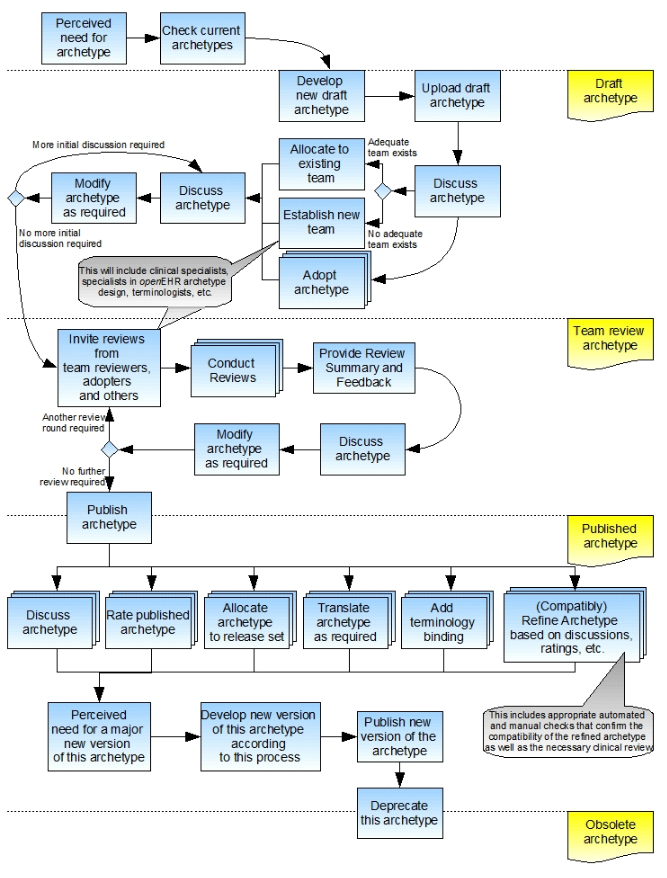
\includegraphics[width=0.95\textwidth]{img/arch_auth.PNG}
	\caption{Archetype authoring, review and publication \citep{Leslie2008}}
	\label{fig:arch_auth}
\end{figure}

TODO\\
TODO\\
TODO\\
TODO\\
TODO\\


\section{Distributed governance of archetypes}
\url{https://www.openehr.org/releases/AM/latest/docs/Identification/Identification.html#_distributed_governance} \\

TODO\\
TODO\\
TODO\\
TODO\\
TODO\\


\end{document}